El aprendizaje automático supervisado, es un enfoque dentro del campo del aprendizaje automático, donde se entrena un modelo utilizando un conjunto de datos etiquetados. En este método, el modelo se entrena para aprender la relación entre las características (variables independientes) y las etiquetas o salidas deseadas (variables dependientes) presentes en los datos de entrenamiento. Como se puede apreciar en la Figura \ref{fig:an8}, donde el conjunto de entrenamiento consiste en mensajes de correo etiquetados como spam o no spam, a partir del cual el modelo podrá predecir a cuál de las dos clases corresponde algún otro correo no etiquetado (nueva instancia). 

\begin{figure}
	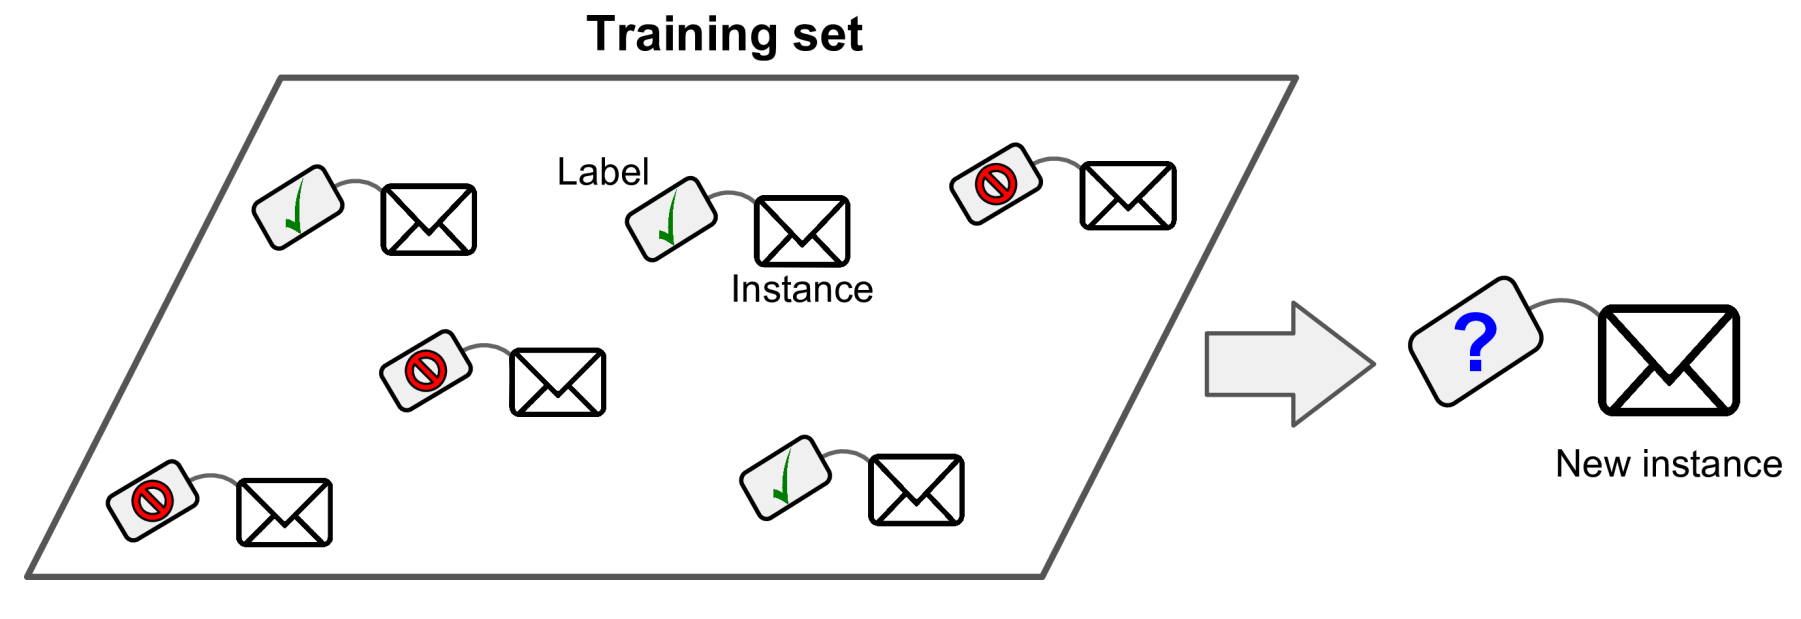
\includegraphics[width=0.65\textwidth]{capitulo2/figuras/an8.png}
	\caption{Un conjunto de entrenamiento etiquetado para aprendizaje supervisado}
	\floatfoot{Fuente: Hands-on machine learning with Scikit-Learn, Keras, and TensorFlow \cite[p. 8]{geron2019hands} }
	\label{fig:an8}
\end{figure}